This chapter is for showing graphically examples of the one-dimensional and two dimensional wavelet transform.  For one dimensional wavelet transform a simple sinusoid signal is used as the source input to measure correctness of the implementation.   Likewise, a simple pictorial image is used as the test input to show correctness of these implementations of the two dimensional wavelet transform.  

\section{Results --- 1D Wavelet Transform}

Testing of the 1D wavelet was performed on a sinusoidal wave form of 128 elements:
\begin{equation}\label{sinusoid}
y(n) = 10 \sin \left({n \over 128}\right) 
	- 5 \sin \left({n \over 64}\right) 
	+ 2 \sin \left({3 n \over 128}\right)
	- \sin \left({n \over 32}\right).
\end{equation}
This function  is the input function used for the one-dimensional implementations and is shown graphically in Figure \ref{sample}. The first test of the 1D transform used the even elements of both convolutions to generate the wavelet transform.  These even elements came from the over-complete form and naturally allow the potential to have complete information.  However, in doing so, a fundamental flaw appears.

\begin{figure}
\begin{center}\includegraphics [width=4in]{sample.jpg} \end{center}
\caption{Sample function.  The $x$-axis is the array index (index $n$).  The $y$ value is simple -- the value $y(n)$. }
\label{sample}
\end{figure}

In order to evaluate the effectiveness of the wavelet transform three
tests have been devised.  First, energy equivalence is used to
determine how much energy is retained in the transform from the
original.  The general shape is used on a the first resolution to test
if the average signal has the same general shape as the original.
Lastly, the inverse transform is used to recover the original signal.
A comparison is made between the original and the recovered signal.

After one resolution, the transformed signal has the same energy as
the original.  This is good since it allows the original to be
recovered from the transform.  Also, the average component of the
transform has the same shape as the original, which is good.  However,
the recovered signal is missing the last element.  Refer to Figure
\ref{recoverEven}. The secret is in which elements are used from the
over-complete to make the complete.  The over-complete form is defined
from the average and difference components which are simply the result
of convolution.

\begin{figure}
\begin{center}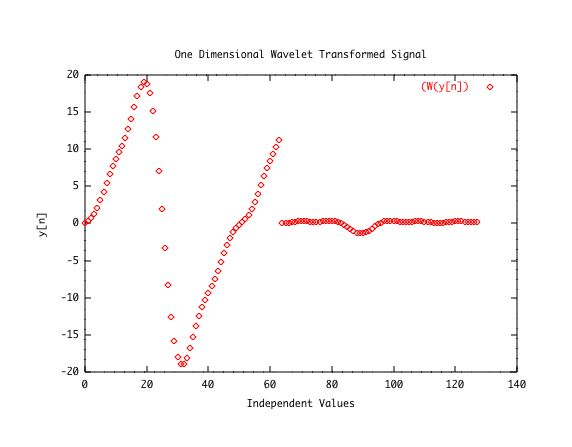
\includegraphics [width=6in]{haar1d.jpg} \end{center}
\caption{\label{wavelet_sample}
Signal after the wavelet transformation.}	
\end{figure}


The convolution means is at the heart of the issue.  The convolution operator in this case starts with the first element of the filter against the first element of the signal.  In the simple Haar Wavelet case, there is a transformation pairing
\[
(S_i , S_{i-1}) \rightarrow A_i, \mbox{ and } (S_i , S_{i-1}) \rightarrow D_i .
\]
In this pairing with zero indexed signals, the odd indexed elements from the over-complete must be used to have all elements of the original accounted for.   

Also this produces a functional difference between wavelet inverse transform for odd and even versions.  The difference is slight; however, the last element is lost in the even indexed form.  
\begin{eqnarray*}
\mbox{Odd: } \qquad R_{2i} =(A_i - D_i ) \sqrt{1/2}, &\qquad& R_{2i+1}=(A_i + D_i ) \sqrt{1/2} \\
\mbox{Even: } \qquad R_{2i} =(A_i + D_i ) \sqrt{1/2}, &\qquad& R_{2i-1}=(A_i - D_i ) \sqrt{1/2} 
\end{eqnarray*}


%The even split  and analysis of this transform.  
\begin{figure}
\begin{center}\includegraphics [width=6in]{recoveredEven.jpg} \end{center}
\caption{Recovered function.  The $x$-axis is the array index (index n).  The $y$ value is simply the value $y(n)$.  The function was recovered from an even indexed wavelet transform. }
\label{recoverEven}
\end{figure}

 
\begin{figure}
\begin{center}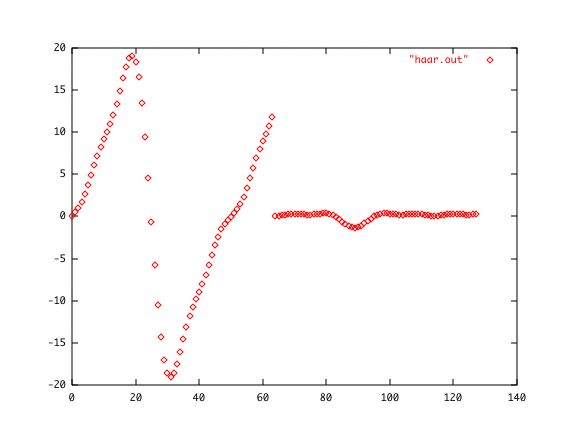
\includegraphics [width=6in]{recovered.jpg} \end{center}
\caption{Recovered function.  The x-axis is the array index (index n).  The y value is simply the value y[n].  The function was recovered from an odd indexed wavelet transform. }
\label{recoverOdd}
\end{figure}

An odd indexed wavelet transform yields the same energy.  However, all of the values are accounted for.  Refer to Figure \ref{recoverOdd}.  

\section {Results: 2D Wavelet Transform }
A simple room picture shows the difference that correct indexing produces in the wavelet transform and its inverse. The 1D to 2D method shows the incorrectly indexed case.  A correctly indexed version is shown in the vector-matrix method.  

The 1D to 2D implementation has a serious issue with memory leak errors.  Memory is allocated and deallocated quickly, and on some platforms shows up as an error.   Some platforms are not forgiving of this error and will force the program to terminate (Macintosh OSX 10.2, using gcc 3.1).    On other platforms, the error is tolerated and performance is degraded (IRIX, SGI Octane2 using gcc 2.9).   An example image of 720 x 486 required nearly 10 minutes to compute the wavelet transform by this method on an SGI Octane2.  However, it does eventually return a correct result.  

The matrix-vector method also yields the correct result.  However, there is less memory overhead in this method as compared to the 1D to 2D method.  As a result, both the row wavelet transform and column wavelet transforms are performed more quickly, with fewer memory transfers and allocations.  Obviously, this also allows for the operation to be conducted almost entirely in cache memory on both the SGI Octane2 and Macintosh G4 based machines.  A Macintosh G3 based machine still requires main memory at a minimum to execute the same operation.% which yields a slower performance.  

A correct result must also be matched to a correct inverse method.  The indexing order matters.  The inverse transform method is a forward inverse transform method.  In the case of 1D to 2D transform, the ordering was reverse indexed (Figure \ref{rightWavepic}).  As a result of an error in indexing, ringing is seen on edges in this method(Figure \ref{rightDanRecovered}) for a case in point.  Caution is incredibly important when matching both forward and reverse indexing, since matching the mathematics to the actual ordering can be obscure and tricky.   

A correct result is shown in Figure \ref{selfRecover}.  In this case, the indexing was matched up and ringing is not present.  It is clear that the recovered image and the original (Figure \ref{rightDan}) are nearly indistinguishable.  

\begin{figure}[htb]
\begin{center}
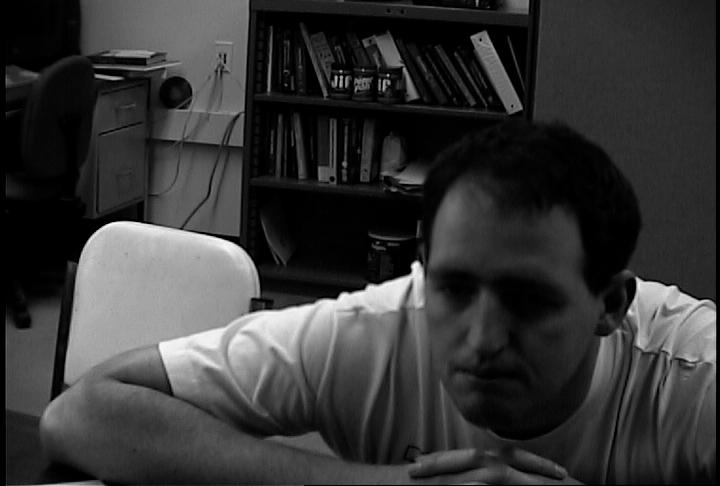
\includegraphics [width=4in]{rightDan.jpg}
\end{center}
\caption{Original Image.  This image is the original image. }
\label{rightDan}
\end{figure}

\begin{figure}[htb]
\begin{center}
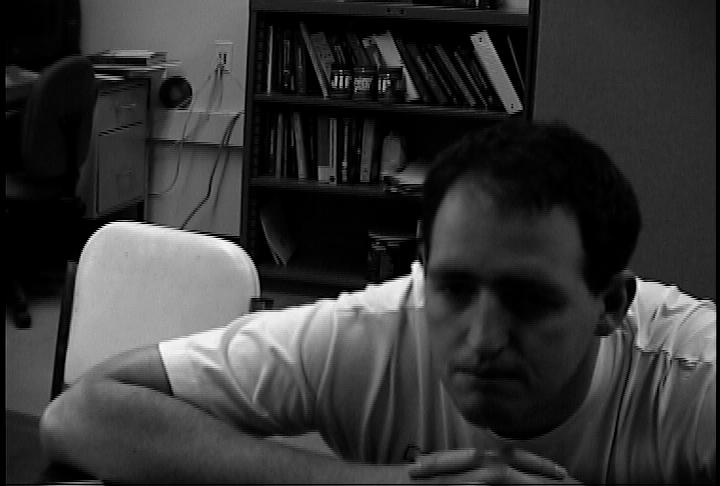
\includegraphics [width=4in]{revRecover.jpg}
\end{center}
\caption{Recovered Image.  This image is the recovered image.  Depending on whether the image was saved as a picture first can affect the white spots in the picture.  Ringing is also an issue.  }
\label{rightDanRecovered}
\end{figure}

\begin{figure}[htb]
\begin{center}
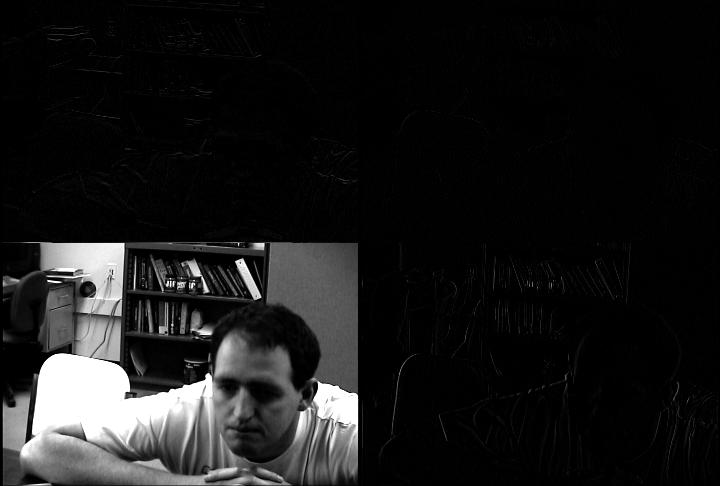
\includegraphics [width=4in]{revWavepic.jpg}
\end{center}
\caption{Wavelet Transform Image.  This image is divided in to average, horizontal, vertical and diagonal components. }
\label{rightWavepic}
\end{figure}

%Note: April 11, 2003:  Proofed up to this point

\begin{figure}[htb]
\begin{center}
\includegraphics [width=4in]{selfWavepic.jpg}
\end{center}
\caption{Wavelet Transform Image.  This image is divided in to average, horizontal, vertical and diagonal components, using the vector-matrix version. }
\label{wavepic}
\end{figure}

\begin{figure}[htb]
\begin{center}
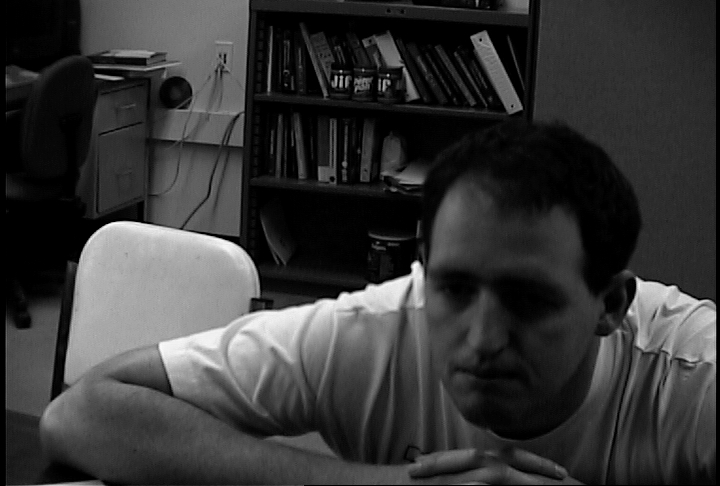
\includegraphics [width=4in]{selfRecover.jpg}
\end{center}
\caption{Recovered Image (Vector-Matrix Method).  This image is the recovered image.  This version avoids the ringing by using the vector-matrix version which is more aligned for the inverse wavelet transform.  }
\label{selfRecover}
\end{figure}


\subsection {Multiresolution Results}
The expected result is a picture within a picture.  Each average component has a further transform on it.  The three resolution transform has the form:
\[
\left(\begin{array}{cccccccc}A_3 & V_3 & V_2 &  & V_1 &  &  &  \\H_3 & D_3 &  &  &  &  &  &  \\H_2 &  & D_2 &  &  &  &  &  \\ &  &  &  &  &  &  &  \\H_1 &  &  &  & D_1 &  &  &  \\ &  &  &  &  &  &  &  \end{array}\right)
\]
%\[
%W_3 = 
%\left(
%\begin{array}{cc}
%\left(
%\begin{array}{cc}
%\left(
%\begin{array}{cc}
%A_3& V_3 \\ 
%H_3 & D_3
%\end{array} 
%\right)
%V_2 \\ 
%H_2 & D_2
%\end{array}
%\right)
% & V_1 \\ 
%H_1 & D_1
%\end{array}
%\right)
%\]
Refer to Figure \ref{wavepicR3} for the image transform results.  

\begin{figure}[htb]
\begin{center}
\includegraphics [width=4in]{wavepic3R.jpg}
\end{center}
\caption{Wavelet Transform Image.  This image is divided in to average, horizontal, vertical and diagonal components using multiresolution wavelet transform.  Note the the average component was transformed one step further. }
\label{wavepicR3}
\end{figure}

\begin{figure}[htb]
\begin{center}
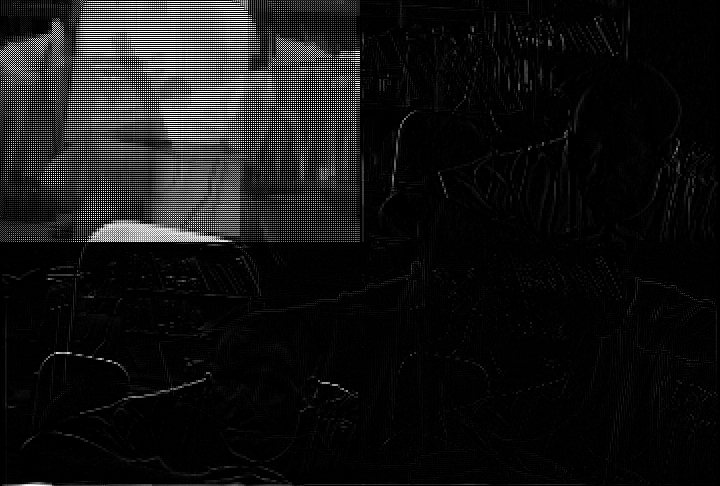
\includegraphics [width=4in]{recoverHid.jpg}
\end{center}
\caption{Recovered Image - Wrong Order (Multiresolution). This image shows a 2D wavelet transform after it was recovered out of order.  Obviously, the distortion is hideous.  }
\label{recoverHid}
\end{figure}

To obtain the inverse, an exact reverse procedure is necessary, otherwise the distortion is hideous.   The first attempt of the wavelet inverse transform was out of order, refer to Figure \ref{recoverHid}.  A correct picture was obtained during the second attempt.  Correct order yielded correct results, refer to Figure \ref{rightDanRecovered}.



\subsection {Threshold Filtering}
After a triple resolution, a 0.02 threshold will eliminate 81.1706 percent of elements in the original sample picture.  Also at this point, the effects of removing these elements becomes visually evident (Figure \ref{recover3R002}).  At a 0.01 threshold,  66.0205 percent of the elements are removed.  Visually, the recovered sample and the original appear to be the same (Figure \ref{recover3R001}).  At a threshold of 0.1, 92.9987 percent of the elements are reduced to zero.  However, the distortions are clearly visible at this level of thresholding (Figure \ref{recover3R010}).  Even at a threshold of 0.001 which is below the numerical precision of the original, 16.0814 elements are reduced to zero.  At a threshold of 0.002, 28.9683 percent is removed.  

Consequently after a triple resolution, nearly 29\% of the data was irrelevant for the image's brightness resolution (which also applies to color).  Subjective examination reveals that removing 60\% to 85\% of the data was not noticeable to human perception.  Which leaves only 15\% to 40\% of the data actually contributing or being necessary to reconstruct the image.   

\begin{figure}[htb]
\begin{center}
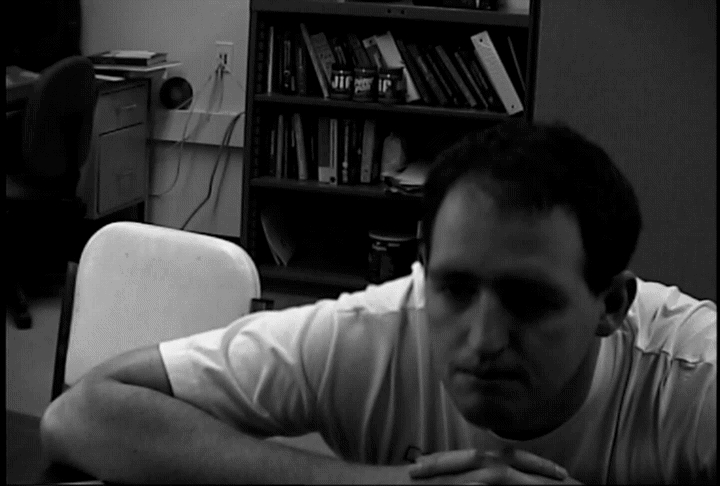
\includegraphics [width=4in]{recover3R002T.jpg}
\end{center}
\caption{Recovered Image - 2\% threshold (Multiresolution). This image had nearly 83\% of its elements removed in the triple resolution wavelet transform.  }
\label{recover3R002}
\end{figure}


\begin{figure}[htb]
\begin{center}
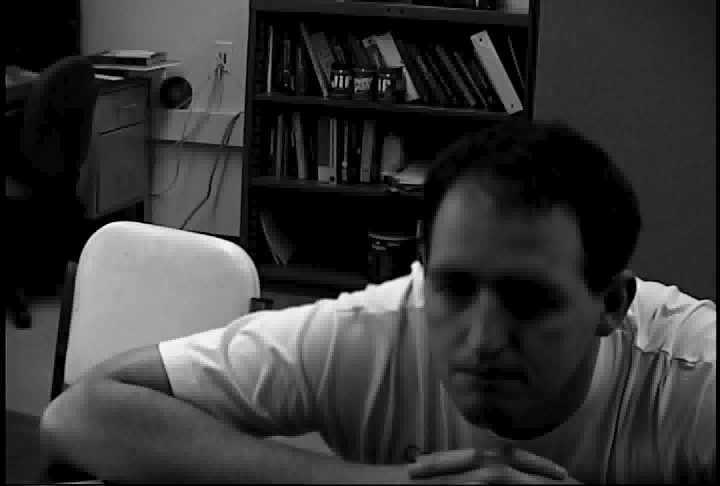
\includegraphics [width=4in]{recover3R010T.jpg}
\end{center}
\caption{Recovered Image - 10\% threshold (Multiresolution). This image had nearly 93\% of its elements removed in the triple resolution wavelet transform.  }
\label{recover3R010}
\end{figure}


\begin{figure}[htb]
\begin{center}
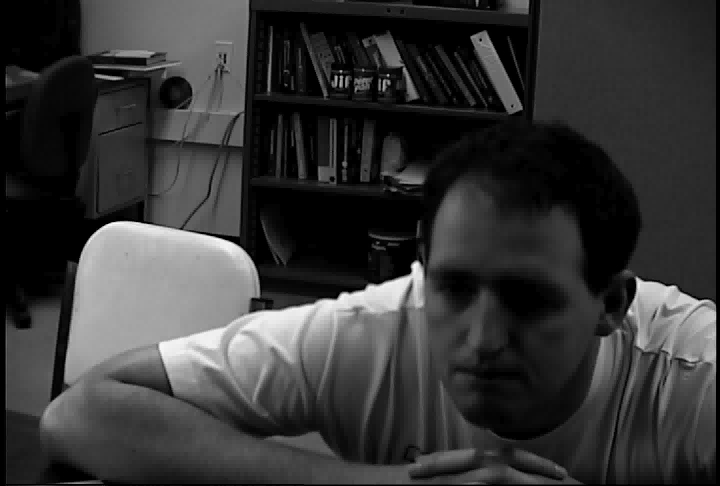
\includegraphics [width=4in]{recover3R005T.jpg}
\end{center}
\caption{Recovered Image - 5\% threshold (Multiresolution). This image had nearly 85\% of its elements removed in the triple resolution wavelet transform.    }
\label{recover3R005}
\end{figure}


\begin{figure}[htb]
\begin{center}
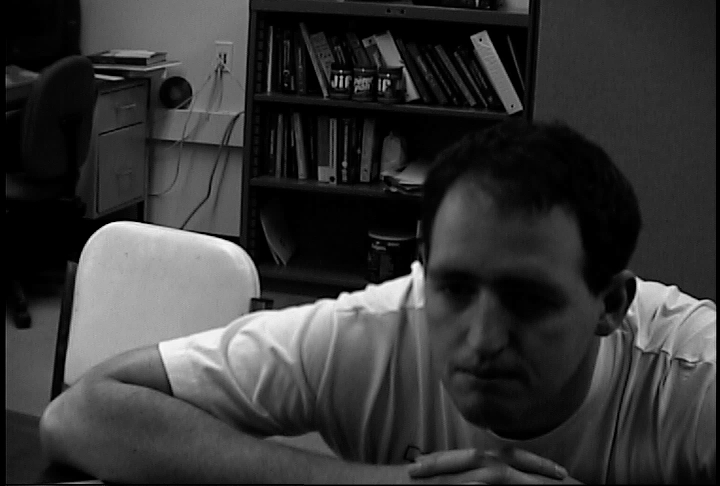
\includegraphics [width=4in]{recover3R001.jpg}
\end{center}
\caption{Recovered Image - 1\% threshold (Multiresolution).  This image had nearly 60\% of its elements removed in the triple resolution wavelet transform.   }
\label{recover3R001}
\end{figure}

